\documentclass[12pt]{article}
\usepackage{url, graphicx}
\usepackage{geometry}
\usepackage{amsmath}
\usepackage{fancyhdr}
\usepackage{nopageno}
\usepackage[usenames, dvipsnames]{color}

\pagestyle{fancy}

\title{\huge Lecture 7: Graph Theory Review}
\author{}
\date{}
\pagestyle{fancy}
\fancyhf{}
\lhead{COMP 251 Winter 2018}
\rhead{Lecture 7}
\lfoot{$22^{nd}$ Jan, 2018}
\rfoot{\copyright{}Yutong Yan}
\newcommand{\forceindent}{\leavevmode{\parindent=1em\indent}}
\begin{document}
\maketitle


\section{Undirected Graphs}
\renewcommand{\labelitemii}{$\circ$}
\renewcommand{\labelitemiii}{$\cdot$}
\renewcommand{\labelitemiii}{$\rightarrow$}
\renewcommand{\labelitemiv}{$\star$}
\begin{itemize}
\item An \underline{undirected} \textbf{graph} $G = (V, E)$ consists of :
	\begin{itemize}
	\item A set V of \textbf{vertices} (or \textbf{nodes}).
	\item A set E of  \textbf{edges} (or \textbf{links}) denoting unordered vertex pairs.
	\end{itemize}
\begin{center}
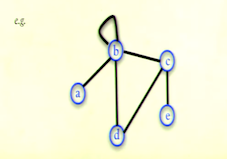
\includegraphics{lecture71}
\end{center}
\item We set $n = |V|$ to be the \underline{cardinality} of the vertex set.
\item We set $m = |E|$ to be the \underline{cardinality} of the edge set.
\end{itemize}


\section{Undirected Graphs}
\renewcommand{\labelitemii}{$\circ$}
\renewcommand{\labelitemiii}{$\cdot$}
\renewcommand{\labelitemiii}{$\rightarrow$}
\renewcommand{\labelitemiv}{$\star$}
\begin{itemize}
\item A \underline{directed} \textbf{graph} $G = (V, E)$ consists of :
	\begin{itemize}
	\item A set V of \textbf{vertices}.
	\item A set A of  \textbf{arcs} (directed edges) denoting \textit{ordered} vertex pairs.
	\end{itemize}
\begin{center}
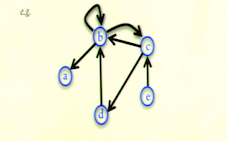
\includegraphics{lecture72}
\end{center}
\item We set $n = |V|$ to be the \underline{cardinality} of the vertex set.
\item We set $m = |A|$ to be the \underline{cardinality} of the arc set.
\end{itemize}

\section{Adjacency Matrix (Undirected Graphs)}
\renewcommand{\labelitemii}{$\circ$}
\renewcommand{\labelitemiii}{$\cdot$}
\renewcommand{\labelitemiii}{$\rightarrow$}
\renewcommand{\labelitemiv}{$\star$}
\begin{itemize}
\item For an \underline{undirected} graph, an \textbf{adjacency matrix} M has the properties that:
	\begin{itemize}
	\item There is a \textbf{row} for each vertex.
	\item There is a \textbf{column} for each vertex.
	\item The ij-th \textbf{entry} of the matrix is defined by:
	\begin{equation*}
  	M_{ij} = \begin{cases}
    	1, & \text{$(i, j) \in E$}.\\
    	0, & \text{$(i, j) \not\in E$}.
  	\end{cases}
	\end{equation*}
	\end{itemize}
\begin{center}
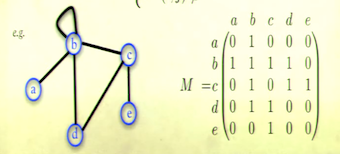
\includegraphics{lecture73}
\end{center}
\end{itemize}


\section{Adjacency Matrix (Directed Graphs)}
\renewcommand{\labelitemii}{$\circ$}
\renewcommand{\labelitemiii}{$\cdot$}
\renewcommand{\labelitemiii}{$\rightarrow$}
\renewcommand{\labelitemiv}{$\star$}
\begin{itemize}
\item For a \underline{directed} graph, an \textbf{adjacency matrix} M has the properties that:
	\begin{itemize}
	\item There is a \textbf{row} for each vertex.
	\item There is a \textbf{column} for each vertex.
	\item The ij-th \textbf{entry} of the matrix is defined by:
	\begin{equation*}
  	M_{ij} = \begin{cases}
    	1, & \text{$(i, j) \in A$}.\\
    	0, & \text{$(i, j) \not\in A$}.
  	\end{cases}
	\end{equation*}
	\end{itemize}
\begin{center}
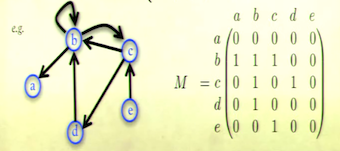
\includegraphics{lecture74}\\
Note: No longer symmetric as undirected graphs!
\end{center}
\end{itemize}



\section{Adjacency Lists (Undirected Graphs)}
\renewcommand{\labelitemii}{$\circ$}
\renewcommand{\labelitemiii}{$\cdot$}
\renewcommand{\labelitemiii}{$\rightarrow$}
\renewcommand{\labelitemiv}{$\star$}
\begin{itemize}
\item An undirected graph can also be stored using \textbf{adjacency lists}.
	\begin{itemize}
	\item For each vertex i, we store a list of the \textbf{neighbours} of i.\\
	Neighbours: the set of vertices that i shares an edge with.
	\item Equivalently, we store a list of the edges \textit{incident} to each vertex.
	\end{itemize}
\begin{center}
	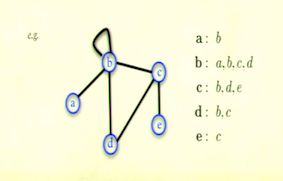
\includegraphics{lecture75}
	\end{center}
\end{itemize}


\section{Adjacency Lists (Directed Graphs)}
\renewcommand{\labelitemii}{$\circ$}
\renewcommand{\labelitemiii}{$\cdot$}
\renewcommand{\labelitemiii}{$\rightarrow$}
\renewcommand{\labelitemiv}{$\star$}
\begin{itemize}
\item A directed graph can also be stored using \textbf{adjacency lists}.
	\begin{itemize}
	\item For each vertex i, we store a list of the \textbf{in-neighbours} of i.
	\item For each vertex i, we store a list of the \textbf{out-neighbours} of i.\\
	In-neighbours: the set of vertices with arcs that point to i.\\
	Out-neighbours: the set of vertices that i has arcs pointing to
	\end{itemize}
	\begin{center}
	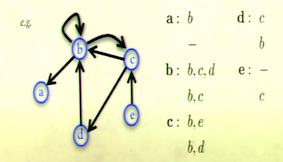
\includegraphics{lecture76}
	\end{center}
\end{itemize}




\section{Adjacency Lists versus Adjacency Matrices}
\renewcommand{\labelitemii}{$\circ$}
\renewcommand{\labelitemiii}{$\cdot$}
\renewcommand{\labelitemiii}{$\rightarrow$}
\renewcommand{\labelitemiv}{$\star$}
\begin{itemize}
\item The main difference is in the amount of \textbf{storage} required
	\begin{itemize}
	\item An \textit{adjacency} matrix requires storing $\Theta(n^2)$ numbers.
	\item An \textit{adjacency} list requires storing $\Theta(m)$ numbers.
		\begin{itemize}
		\item Each arc will appear twice in a list. 
		\end{itemize}
	\end{itemize}
\item In any graph $m = O(n^2)$ and often $m \ll n^2$
	\begin{itemize}
	\item In \textbf{sparse graphs} it is much more preferable to use adjacency lists.
	\end{itemize}
\end{itemize}



\section{Graph Application}
\renewcommand{\labelitemii}{$\circ$}
\renewcommand{\labelitemiii}{$\cdot$}
\renewcommand{\labelitemiii}{$\rightarrow$}
\renewcommand{\labelitemiv}{$\star$}
\begin{itemize}
\item The number of practical applications for is very large.
\item Obviously there are useful in modelling \underline{networks}.
	\begin{itemize}
	\item Transportation Networks: e.g. Roads.
	\item Social Networks: e.g. Facebook Graph.
	\item Information Networks: e.g. the World Wide Web.
	\item Financial Networks: e.g. Monetary Flows.
	\end{itemize}
\item But, their flexibility allows them to model a plethora of diverse applications:
	\begin{itemize}
	\item Hierarchy: data structures, linguistics.
	\item Similarity: data clustering, biology.
	\item Conflict: wavelength allocation, scheduling.
	\item Priority: industrial planning, operations research.
	\item Structure: chemistry, physics.
	\item Time Relations: evolution, migration patterns.
	\end{itemize}
\end{itemize}


\section{Graph Structure}
\renewcommand{\labelitemii}{$\circ$}
\renewcommand{\labelitemiii}{$\cdot$}
\renewcommand{\labelitemiii}{$\rightarrow$}
\renewcommand{\labelitemiv}{$\star$}
\begin{itemize}
\item Walks
	\begin{itemize}
	\item A \textbf{walk} is list of vertices $\{v_0, v_1, ... , v_l\}$ such that $(v_i, v_{i+1}) \in E$ for all $0 \leq i < l.$
	\end{itemize}
\begin{center}
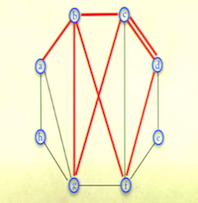
\includegraphics{lecture77}
\end{center}

\item Circuits
	\begin{itemize}
	\item A \textbf{circuit} is a walk $\{v_0, v_1, ... , v_l\}$ where $v_0 = v_l$.
	\item A circuit is a \textbf{closed} walk.
	\item We are not allowed to use same edge/arc more than once.
	\item An \textbf{Eulerian Circuit} is a circuit that uses every edge exactly once.
	\end{itemize}
\begin{center}
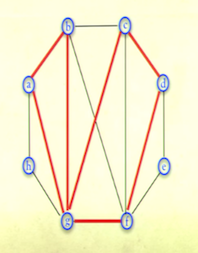
\includegraphics{lecture78}
\end{center}
	
\item Paths
	\begin{itemize}
	\item A \textbf{path} is a walk where every vertex is \underline{distinct}.
	\item Revisit is not allowed.
	\end{itemize}	
\begin{center}
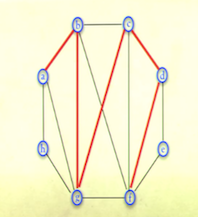
\includegraphics{lecture79}
\end{center}


\item Cycles
	\begin{itemize}
	\item A \textbf{cycle} is a walk $\{v_0, v_1, ... , v_l\}$ where every vertex is \underline{distinct} except for the end-vertices $v_0 = v_l$.
	\item A cycle is a \textbf{closed} path.
	\item An \textbf{Hamiltonian Cycle} is a cycle that uses every vertex exactly once.
	\end{itemize}	
\begin{center}
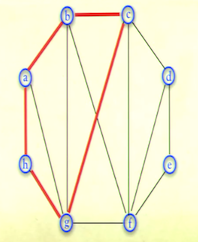
\includegraphics{lecture710}
\end{center}
\end{itemize}

\section{Connected Graphs}
\renewcommand{\labelitemii}{$\circ$}
\renewcommand{\labelitemiii}{$\cdot$}
\renewcommand{\labelitemiii}{$\rightarrow$}
\renewcommand{\labelitemiv}{$\star$}
\begin{itemize}
\item A graph is \textbf{connected} if for every pair of vertices $u, v \in V$, it is possible to walk from u to v.
\item A graph is \textbf{disconnected} if there exists a pair of vertices $u, v \in V$, for which there is no possible walk from u to v.
\end{itemize}
\begin{center}
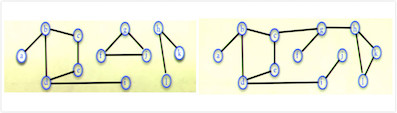
\includegraphics{lecture711}
\end{center}
\begin{itemize}
\item Graph Components
	\begin{itemize}
	\item A connected subgraphs are called the \textbf{components} of the graph.
	\item Thus a connected graph has exactly \underline{one} component.
	\end{itemize}
\end{itemize}
\begin{center}
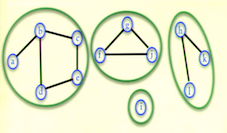
\includegraphics{lecture712}
\end{center}

\section{Trees}
\renewcommand{\labelitemii}{$\circ$}
\renewcommand{\labelitemiii}{$\cdot$}
\renewcommand{\labelitemiii}{$\rightarrow$}
\renewcommand{\labelitemiv}{$\star$}
\begin{itemize}
\item A \textbf{tree} is a connected component with no cycles.
\item A \textbf{forest} is a graph whose components are all trees.
\item A tree is \textbf{spanning} if it contains every vertex in the graph.
\end{itemize}
\begin{center}
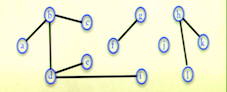
\includegraphics{lecture713}
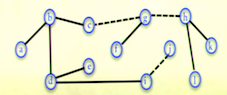
\includegraphics{lecture714}
\end{center}

\section{Matchings}
\renewcommand{\labelitemii}{$\circ$}
\renewcommand{\labelitemiii}{$\cdot$}
\renewcommand{\labelitemiii}{$\rightarrow$}
\renewcommand{\labelitemiv}{$\star$}
\begin{itemize}
\item A \textbf{matching} is a set of vertex-disjoint edges.
\item Hence, each vertex is incident to at most one edge in the matching.
\item A matching is \textbf{perfect} if every vertex is incident to an edge in the matching.
\end{itemize}
\begin{center}
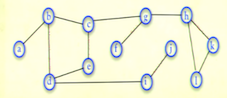
\includegraphics{lecture716}
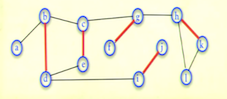
\includegraphics{lecture715}
\end{center}

\section{Cliques}
\renewcommand{\labelitemii}{$\circ$}
\renewcommand{\labelitemiii}{$\cdot$}
\renewcommand{\labelitemiii}{$\rightarrow$}
\renewcommand{\labelitemiv}{$\star$}
\begin{itemize}
\item A \textbf{clique} is a set of pairwise adjacent vertices.
\end{itemize}
\begin{center}
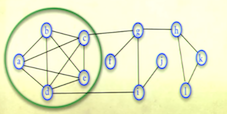
\includegraphics{lecture717}
\end{center}


\section{Independent Sets}
\renewcommand{\labelitemii}{$\circ$}
\renewcommand{\labelitemiii}{$\cdot$}
\renewcommand{\labelitemiii}{$\rightarrow$}
\renewcommand{\labelitemiv}{$\star$}
\begin{itemize}
\item An \textbf{independent set (stable set)} is a set of pairwise non-adjacent vertices.
\item If you find a stable set, then there is no conflict. (Assume the graph representing conflicts.)
\end{itemize}
\begin{center}
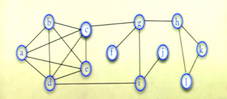
\includegraphics{lecture718}\\
(c, f, j, l)
\end{center}



\section{Bipartite Graphs}
\renewcommand{\labelitemii}{$\circ$}
\renewcommand{\labelitemiii}{$\cdot$}
\renewcommand{\labelitemiii}{$\rightarrow$}
\renewcommand{\labelitemiv}{$\star$}
\begin{itemize}
\item In a \textbf{bipartite graph} the vertex set can be partitioned as $V = X \cup Y$ such that every edge has one end-vertex in $X$ and one end-vertex in $Y$.
\end{itemize}
\begin{center}
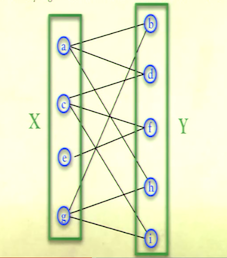
\includegraphics{lecture719}\\
Note that X and Y are both independent sets.
\end{center}




\section{Some Theorems on Undirected Graphs}
\renewcommand{\labelitemii}{$\circ$}
\renewcommand{\labelitemiii}{$\cdot$}
\renewcommand{\labelitemiii}{$\rightarrow$}
\renewcommand{\labelitemiv}{$\star$}
\begin{itemize}
\item The Handshaking Lemma	
	\begin{itemize}
	\item Let $\tau (v) = \{u: (u,v) \in E\}$ be the set of neighbours of v.
	\item The degree, $deg(v)$, of a vertex v is the cardinality of $\tau (v)$.
	\end{itemize}
\textbf{The Handshaking Lemma.} In an undirected graph, there are an even number of vertices with odd degree.\\
\textbf{Proof.} 
\begin{itemize}
\item We have: \\
	$$2 \cdot |E| = \sum_{v \in V} deg(v)$$
	\begin{center} (Double count the number of pairs (v,e) where e is an edge incident to v.) \end{center}
	$$= \sum_{v \in O} deg(v) + \sum_{v \in \varepsilon} deg(v)$$
	\begin{center} ($O$ is the set of vertices with odd degree, and $\varepsilon$ is the set of vertices with even degree.) \end{center}
	$$ \Rightarrow \sum_{v \in O} deg(v) = 2 \cdot |E| - \sum_{v \in \varepsilon} deg(v)$$
	\begin{center} Even = Even - Even \end{center}
\end{itemize}
\end{itemize}

\section{Euler's Theorem}
\renewcommand{\labelitemii}{$\circ$}
\renewcommand{\labelitemiii}{$\cdot$}
\renewcommand{\labelitemiii}{$\rightarrow$}
\renewcommand{\labelitemiv}{$\star$}
\begin{itemize}
\item The first result in Graph Theory is the following.\\
\textbf{Theorem.} An undirected graph contains an Euler Circuit if and only if every vertex has an even degree.\\
\textbf{Proof.} Exercise! (Use induction.)
\end{itemize}

\section{A Theorem on Trees}
\renewcommand{\labelitemii}{$\circ$}
\renewcommand{\labelitemiii}{$\cdot$}
\renewcommand{\labelitemiii}{$\rightarrow$}
\renewcommand{\labelitemiv}{$\star$}
\begin{itemize}
\item Leaves
	\begin{itemize}
	\item A vertex with degree one in a tree is called a \textbf{leaf.}\\
	\textbf{Lemma.} A tree T with $n \geq 2 $ vertices has at least one leaf vertex.\\
	\textbf{Proof.}
	\begin{itemize}
	\item A tree is connected $\Rightarrow$ There are \underline{no} vertices with degree 0 as $n \geq 2.$
	\item For a contradiction, assume every vertex has degree at least 2.
	\item Take the \textbf{longest path} $P = \{v_1,v_2,...,v_{l-1},v_l\}$ in T.
	\item But $deg(v_k) \geq 2$ so $v_l$ has a neighbour $x \neq v_{l-1}$
	\item We must have $x = v_j$ for some $1 \leq j \leq l-2$ otherwise $\{v_1, v_2, ... , v_l, x\}$ is a longer path than P.
	\item But then $C = \{x= v_j, v_{j+1}, ..., v_l, x\}$is a cycle, contradiction.
	\end{itemize}
	\end{itemize}
\begin{center}
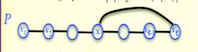
\includegraphics{lecture720}\\
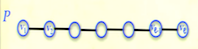
\includegraphics{lecture721}\\
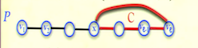
\includegraphics{lecture722}
\end{center}
\item The Number of Edges in a Tree\\
\textbf{Theorem.}  A tree with n vertices has n-1 edges.\\
\textbf{Proof.}
	\begin{itemize}
	\item Let's prove this by induction.
	\end{itemize}
\underline{Base Case:}
	\begin{itemize}
	\item A tree on \textbf{one} vertex has \textbf{zero} edges.
	\end{itemize}
\underline{Induction Hypothesis:}
	\begin{itemize}
	\item Assume that any tree on n-1 vertices has n-2 edges.
	\end{itemize}
\underline{Induction Step:}
	\begin{itemize}
	\item Take a tree T with $n \geq	 2$ vertices.
	\item By the previous lemma, this tree contains a \textbf{leaf} vertex v.\\
	 $\Rightarrow$ T  $\backslash$ \{v\} is a tree on n-1 vertices.\\
	 $\Rightarrow$ By the induction hypothesis, T  $\backslash$ \{v\} is a tree on n-2 vertices.\\
	 $\Rightarrow$ T is a tree with n-1 edges.
	\end{itemize}
\end{itemize}



\section{Hall's Theorem}
\renewcommand{\labelitemii}{$\circ$}
\renewcommand{\labelitemiii}{$\cdot$}
\renewcommand{\labelitemiii}{$\rightarrow$}
\renewcommand{\labelitemiv}{$\star$}
\begin{itemize}
\item How do we know if a bipartite graph $G = (X \cup Y, E)$ contains a \textbf{perfect matching}?
\item This is actually easy to test using Hall's Condition.
\begin{center}
\underline{Hall's Condition:} $\forall B \subseteq X$, $|\tau(B)| \geq |B|$
\end{center}
\textbf{Hall's Theorem.}  A bipartite graph, with $|X| = |Y|$, contains a perfect matching if and only if Hall's condition is satisfied.\\
\textbf{Proof.}\\
($\Rightarrow$)
	\begin{itemize}
	\item If there is a set $B \subseteq X$ with $|\tau(B)| < |B|$ then the graph \textbf{cannot} have a perfect matching.
	\end{itemize}
($\Leftarrow$)
	\begin{itemize}
	\item Suppose Hall's Condition is satisfied: $\forall B \subseteq X$, $|\tau(B)| \geq |B|$
	\item Take a \textbf{maximum cardinality} matching M in the graph.
	\item If M is perfect we are done.
	\item So we may assume M is not perfect and there is an \textbf{unmatched} vertex $b_0$ in $X$.
	\item As Hall's condition holds we have: $|\tau(\{b_0\})| \geq |\{b_0\}| = 1$
	\item So $b_0$ has at least one neighbour $s_0$
	\item Let $s_0$ be matched to $b_1$ in M
	\item As Hall's condition holds we have: $|\tau(\{b_0, b_1\})| \geq |\{b_0, b_1\}| = 2$
	\item So either $b_0$ or $b_1$ has a neighbour $s_1 \neq s_0$
	\item Let $s_1$ be matched to $b_2$ in M.
	\item As Hall's condition holds we have: $|\tau(\{b_0, b_1, b_2\})| \geq |\{b_0, b_1, b_2\}| = 3$
	\item So either $\{b_0, b_1, b_2\}$ has a neighbour $s_2  \neq \{s_0, s_1\}$
	\item As Hall's condition holds we have: $|\tau(\{b_0, b_1, b_2, b_3\})| \geq |\{b_0, b_1, b_2, b_3\}| = 4$
	\item So either $\{b_0, b_1, b_2, b_3\}$ has a neighbour $s_3  \neq \{s_0, s_1, s_2\}$\
	\item ...
	\item The graph contains a finite number of nodes so this process must terminate.
	\item The process can only terminate if we reach an unmatched node  $s_k \in S$
	\item Using the edges we have found we can trace back a \textbf{path} P from $s_k$ to $b_0$ that alternates between using non-matching edges and matching edges.
	\item \textbf{Swapping} the matching and non-matching edges gives one extra matching edge.
	\item Note this is still a \underline{valid} matching. Firstly, the internal nodes of P are still incident to exactly one matching edge.
	\item Secondly, its end-nodes, $s_k$ and $b_0$, were previously unmatched so are now incident to exactly one edge in the new matching.
	\item This contradicts the fact that M was a maximum cardinality matching.
	\begin{center}
	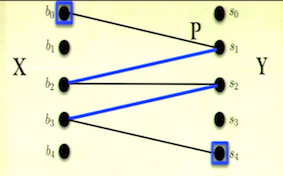
\includegraphics{lecture723}
	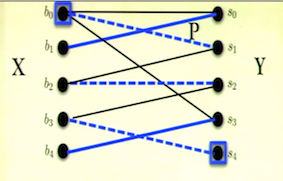
\includegraphics{lecture724}
	\end{center}
	\end{itemize} 
\end{itemize}










\end{document}